\chapter{导览：望远镜到底记录了什么，本书要带你去哪里}
\label{chap:e00}

\begin{chapteropening}
今晚，一颗恒星的光走了几百年才落到镜面上。你可能以为望远镜会替你把它存成一张照片——其实不会。望远镜最终写进硬盘的，既不是一束连续起伏的电磁波，也不是一张已经有物理解释的图像，而是一长串带标签的探测事件：某时刻、某像素、某频道、某通道、又一次“咔哒”。本章不推公式，只做两件事——先带你看清这串“咔哒”里到底藏着什么，再摊开一张全书地图，告诉你我们要一起走到哪里、为什么值得走。
\end{chapteropening}

\section{望远镜到底把光存成了什么}
\label{sec:e00-event}

先纠正一个几乎所有人都有的错觉。我们习惯说“望远镜拍到了一张星图”，好像镜面后面坐着一位画家，实时把天空临摹下来。真实情况要朴素得多，也有趣得多：现代探测器（无论是 CCD 的一个像素、光电倍增管 PMT、还是雪崩二极管 APD、单光子雪崩管 SPAD）本质上都是一台“计数器”。光子撞上来，它“咔哒”记一笔；再撞一个，再记一笔。它不画画，它数数。

所以，一台望远镜在最底层交给我们的，不是图像，而是一张\textbf{事件表}（event list）：每一行对应一次光子探测，每一行都挂着几个标签。把第 \(j\) 次探测写成一行数据，就是

\begin{equation}
  e_j=\bigl(t_j,\;\bm r_j,\;\nu_j,\;p_j,\;w_j\bigr).
  \label{eq:e00-event}
\end{equation}
\begin{formulaexplain}
\(e_j\) 是第 \(j\) 次光子探测这一行数据；\(t_j\) 是它到达的时刻，\(\bm r_j\) 是它落在哪个望远镜/像素，\(\nu_j\) 是它属于哪个频率通道，\(p_j\) 是偏振或电子学通道，\(w_j\) 是这次事件的质量权重。整句话在说：一次“咔哒”被写成一行可以分析的数据。
\end{formulaexplain}

这行式子看着抽象，其实每个标签都很具体，我们逐个拆开：

\begin{itemize}
  \item \(t_j\)——\textbf{到达时间}。这是探测器盖上的时间戳，单位可以是秒、毫秒，也可以精细到纳秒（\(\mathrm{ns}=10^{-9}\,\mathrm{s}\)）甚至皮秒（\(\mathrm{ps}=10^{-12}\,\mathrm{s}\)）。别小看这一列：后面你会看到，正是它把“光子怎样一起到达”这件事变成可测量的物理。
  \item \(\bm r_j\)——\textbf{位置标签}。它可以是一块 CCD 上的像素坐标 \((x,y)\)，也可以是“这个光子被第几号望远镜收到”。当我们谈干涉、谈两台相隔百米的望远镜时，\(\bm r_j\) 就是那对望远镜的编号。
  \item \(\nu_j\)——\textbf{频率通道}（frequency channel）。它记录这个光子大致属于哪一段颜色，单位是 Hz 或干脆是通道号。可见光的频率大约在 \(4\times10^{14}\) 到 \(8\times10^{14}\,\mathrm{Hz}\)，滤光片或光谱仪把这条宽带切成若干窄格，\(\nu_j\) 就是它落进的那一格。
  \item \(p_j\)——\textbf{偏振或电子学通道}（polarization / electronics channel）。它可能是“水平还是垂直偏振”，也可能只是“从哪条读出电路出来的”。这一列常被传统数据丢掉，但它藏着辐射机制和磁场几何的线索。
  \item \(w_j\)——\textbf{质量权重}（weight）。它是我们对这次事件的“信任度”：这一发是不是撞在坏像素上？是不是紧挨着死时间（dead time）？是不是可能来自云层或背景？我们不粗暴地扔掉可疑事件，而是给它一个权重，让后面的统计自己去衡量。它是个\textbf{无量纲}数，通常归一化到 \(0\)（完全不信任、等于把这次事件剔除）到 \(1\)（完全采信）之间，介于其间的取值表示“打个折扣采用”。
\end{itemize}

请记住这张事件表的样子——它是全书真正的主角。传统天文学之所以强大，是因为它懂得从这张表里榨出图像、光谱和光变曲线；而本书想告诉你的是：这张表里还剩下一些东西，传统的“求平均”动作恰好把它们抹掉了。要看见那些剩下的东西，我们必须一次次回到式~\eqref{eq:e00-event} 这一行行原始的“咔哒”。

\section{同一批光子，能被投影成许多种产品}
\label{sec:e00-projection}

事件表最迷人的地方在于：\textbf{同一批光子，可以被投影成完全不同的数据产品}，就像同一束阳光穿过不同形状的窗棂，在地板上投出不同的图案。我们平时熟悉的每一种天文“图”，其实都只是对式~\eqref{eq:e00-event} 沿某一列做的一次分箱（binning）：

\begin{itemize}
  \item 按\textbf{位置} \(\bm r_j\) 分箱——把落在同一片天区的光子数堆在一起，就得到一幅\textbf{图像}。哪里亮，就是哪里的“咔哒”多。
  \item 按\textbf{频率} \(\nu_j\) 分箱——把落在同一颜色格子里的光子数排开，就得到一条\textbf{光谱}。谱线的凹凸，就是某些频道计数的多寡。
  \item 按\textbf{时间} \(t_j\) 分箱——把每一小段时间里的光子数依次列出，就得到一条\textbf{光变曲线}。星星忽明忽暗，就是各时间格里计数的起伏。
  \item 按\textbf{偏振通道} \(p_j\) 组合——把不同偏振通道的强度按规则加加减减，就得到\textbf{偏振量}（Stokes 参数）。
\end{itemize}

关键的一句话要说三遍：\textbf{每一次投影，都保留一部分信息，同时丢掉一部分信息}。当你为了画一幅图，把某个像素里几百万个光子“压”成一个亮度数字时，你确实得到了“这里有多亮”，却永远抹掉了“这几百万个光子是不是喜欢成群结队地一起到达”。当你为了画光变曲线，把每毫秒的光子压成一个计数时，你也就再也分不清同一毫秒里的光子是彼此独立地零星落下，还是在某几微秒里挤成一簇。

这就是本书反复要做的动作：\textbf{在投影之前，先停下来问一句——我正打算丢掉什么？} 有些天体物理问题，投影成图像就够了；但恒星的角直径、黑洞边缘的结构、某些新物理的信号，恰恰藏在那些“被平均掉”的、光子与光子之间的联合关系里。一旦先平均，就再也捞不回来。图~\ref{fig:e00-event-map} 把这件事画成了一张地图：中间是同一张事件表，四面伸出去的，是它能变成的各种产品。

\begin{figure}[tbp]
\centering
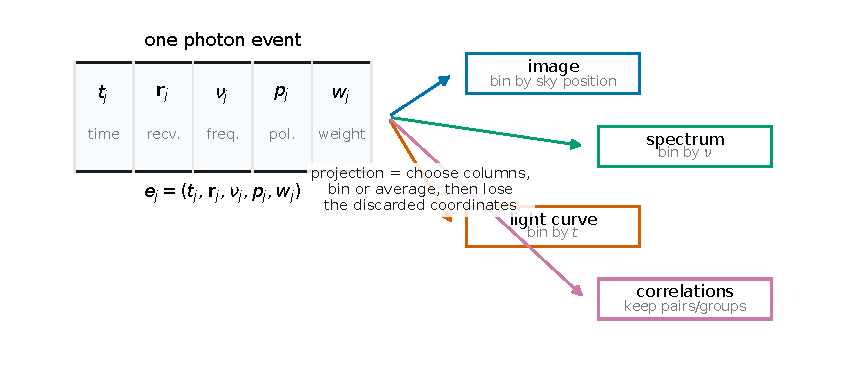
\includegraphics[width=0.9\linewidth]{figures/generated/chapter_01/ch01_event_table_map.pdf}
\caption{同一张光子事件表可以被投影成许多种数据产品。沿位置分箱得到图像，沿频率分箱得到光谱，沿时间分箱得到光变曲线，沿偏振通道组合得到偏振量。每一次投影都保留一部分信息、丢掉一部分信息；而“光子如何两两一起到达”这类关系，只有回到原始事件表才看得见。}
\label{fig:e00-event-map}
\end{figure}

\section{光有两种语言：波，与计数}
\label{sec:e00-two-languages}

要读懂事件表里“被丢掉的东西”，你得先接受一件让物理学家争论了一个世纪的事：\textbf{光同时说着两种语言}，而这两种语言描述的是同一件事。

第一种是\textbf{波的语言}。在一段足够窄的颜色里，光可以被看成一列振荡的电磁波：真正在抖动的是电场，它有振幅、有相位、会干涉。把两束光叠在一起，波峰对波峰就更亮，波峰对波谷就变暗——这就是相长与相消。相位、干涉、条纹，是这门语言的关键词。可见光的电场每秒要振荡上百万亿次，一个周期只有几飞秒（\(\mathrm{fs}=10^{-15}\,\mathrm{s}\)），快到任何普通探测器都跟不上；于是探测器看不见电场的正负摆动，只能把这些飞快的振荡在自己的响应时间里抹平，最后留下能量。

第二种是\textbf{计数的语言}。探测器留下的是一个个离散的“咔哒”，每一次都是一个光子的点击。既然是一次次独立的随机点击，计数就必然带有涨落：哪怕天体亮度、望远镜、探测器都纹丝不动，你数出来的每毫秒光子数也会上下抖动。这种与生俱来的抖动叫\textbf{散粒噪声}（shot noise，也叫泊松噪声），它不是仪器不好，而是“光本来就是一颗颗数出来的”这件事的必然影子。

这两种语言听起来南辕北辙——一个讲连续的波和相位，一个讲离散的点击和概率——但量子天文学的全部魅力，就在于它们其实是同一枚硬币的两面，而且能在\textbf{事件表}里被同时读出来。这里我先只做一个预告，把三条线索埋下：

\begin{itemize}
  \item 波的语言（电场、复振幅、相位、干涉）会在第~\ref{chap:e01} 章被正式接上，我们会把电场写成一支“旋转的箭头”；紧接着第~\ref{chap:e02} 章用傅里叶分析把它延伸开来，讲清带宽与相干时间——也就是“这支箭头能记住自己相位多久”。
  \item 计数的语言（概率、泊松统计、散粒噪声）会在第~\ref{chap:e03} 章被讲透，我们会从最朴素的“把时间切成许多小格”一路推到泊松分布，把“咔哒”的涨落算成一个可预言的数。
  \item 有了这两门语言，我们还要先把“光子”本身讲严谨：第~\ref{chap:e04} 章补上量子力学与谐振子的阶梯算符，第~\ref{chap:e05} 章据此给出光的量子化。这才是把“波”和“计数”真正缝在同一套数学里的针线。
  \item 而把这两种语言彻底焊在一起、让“波的相干”直接变成“计数的关联”的那座桥——强度干涉与 Hanbury Brown--Twiss（HBT）效应——属于全书第 2 部“相干与关联”，要到那里、也就是比光的量子化更靠后的章节，才正式搭起来。
\end{itemize}

换句话说，本章埋下的悬念——“同一批光子怎样一起到达，藏着什么”——它的答案要靠这两种语言合起来才能说清。第~\ref{chap:e01} 到第~\ref{chap:e05} 章先把两门语言各自打磨锋利、并把“光子”定义严谨；真正让二者合流的 HBT 关联，则留到后面的“相干与关联”部分去收网。

\section{本书的承诺：为什么值得学这门“量子”语言}
\label{sec:e00-promise}

你也许会问：传统天文学已经能给出图像、光谱、光变和偏振，日子过得好好的，为什么还要费劲去学这套“回到事件表、盯着光子怎样一起到达”的量子语言？因为它能做到一些传统方法\textbf{原理上做不到}的事。这不是把“量子”当噱头，而是有真金白银的科学回报。

\textbf{测量恒星的真实大小。} 恒星离我们太远，在望远镜里几乎都只是一个点。它们的角直径（angular diameter）小到毫角秒（milliarcsecond, mas，即 \(10^{-3}\) 角秒）乃至微角秒的量级。这有多小？\(1\,\mathrm{mas}\approx4.85\times10^{-9}\,\mathrm{rad}\)，要让一枚直径约 \(2.5\,\mathrm{cm}\) 的硬币张成这么小的角，你得把它放到约五千公里外——差不多是北京到伦敦一半的距离；而微角秒还要再小一千倍。普通望远镜受衍射极限所限根本看不出这么小的角结构，但强度干涉能把两台相隔百米、公里的望远镜的光子计数关联起来，从“两台望远镜的涨落有多同步”里反推出这个角直径。恒星不再是一个点，而有了可测量的圆盘、有了被自转压扁的形状、有了边缘的昏暗。

\textbf{逼近黑洞与致密天体的边缘。} 更长的基线、更高的时间分辨，原则上能把这套方法推向更小的角尺度，去约束吸积盘、恒星风、乃至致密天体周围的结构。

\textbf{给新物理套上绳索。} 光子到达时间与关联的极端精确测量，还能被用来检验一些超出标准模型的设想。凡是能写成“事件表里的一个可估计量 + 一份诚实的误差预算 + 一个 null test”的问题，都可能成为一个真正可执行的观测项目。

这些不是纸上谈兵。请记住三个真实的名字，它们会在全书反复出现：

\begin{itemize}
  \item \textbf{Narrabri}——上世纪六十年代，澳大利亚 Narrabri 的恒星强度干涉仪用两台可以在轨道上滑动的大反射器，第一次系统地量出了几十颗亮星的角直径。这是这门手艺的起点。
  \item \textbf{VERITAS} 与 \textbf{MAGIC}——如今，本为捕捉高能伽马射线而建的大型切伦科夫望远镜阵列（每台口径十几米），被巧妙地改造成光学强度干涉仪，测出了亮星亚毫角秒级的角直径，精度好到几个百分点。当年因信号太弱而沉寂多年的方法，靠着大镜面、高速电子学和数字关联器，重新活了过来。
\end{itemize}

图~\ref{fig:e00-science-map} 把这些科学目标摆在同一张地图上：横看是“离常规观测有多近”，纵看是“能带来多少传统方法拿不到的新信息”。亮星角直径已经近在咫尺，而更远处，是超新星测距、量子网络望远镜这样价值极高、也更需要工程突破的目标。这张图，就是本书想邀请你一起去探索的疆域。

\begin{figure}[tbp]
\centering
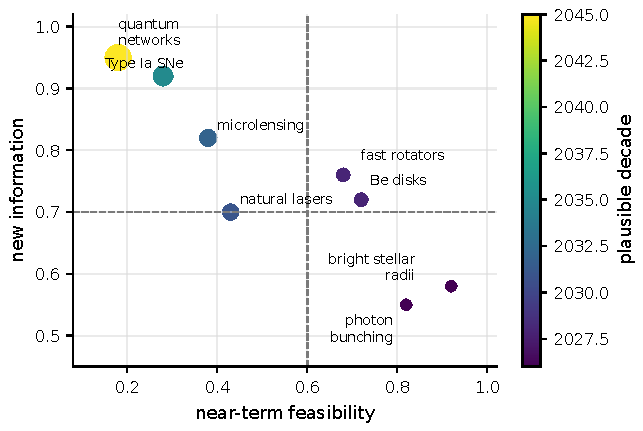
\includegraphics[width=0.8\linewidth]{figures/generated/chapter_02/ch02_science_case_map.pdf}
\caption{量子天文学第一代科学问题的地图：横轴大致表示离常规观测的远近，纵轴表示相对传统方法新增的信息量。亮星角直径和恒星光子聚束已经贴近现有能力；快速自转星、恒星盘、自然激射是近期扩展；超新星角距离测距、量子网络望远镜价值最高，但需要更长基线、快速触发或量子链路等工程突破。}
\label{fig:e00-science-map}
\end{figure}

\section{全书地图：我们要一起走的七站}
\label{sec:e00-map}

最后，摊开整张地图。本书分成七个部分（第 0 到第 6 部），像一条从地基一路盖到屋顶的施工路线。你不必一口气读完，但最好知道每一站在盖哪一层：

\begin{itemize}
  \item \textbf{第 0 部——地基与语言。} 就是你正在读的这几章。我们打磨两件工具：波的语言（电场、复振幅、相位、干涉）和计数的语言（泊松统计、散粒噪声、数量级估算）。目标是让你在遇到任何一条公式时，都先看得见它背后的物理画面。
  \item \textbf{第 1 部——光的量子描述。} 把“光子”这个词讲严谨：从电场的量子化，到相干态（coherent state）、热态（thermal state）与数态，理解为什么激光般的相干光和恒星般的热光，在“光子怎样一起到达”上如此不同。
  \item \textbf{第 2 部——相干与关联。} 本书的心脏。一阶相干 \(g^{(1)}\)（干涉、可见度）与二阶相干 \(g^{(2)}\)（光子聚束、强度关联）在这里登场，Siegert 关系把二者焊接起来，HBT 效应从“怪异现象”变成“可算的物理”。
  \item \textbf{第 3 部——从关联到成像。} van Cittert--Zernike 定理告诉我们，天空的亮度分布如何编码进空间相干度；于是“两台望远镜的关联”被翻译成“恒星的角直径”，强度干涉成像的原理在此闭环。
  \item \textbf{第 4 部——测量的极限。} 引入 Fisher 信息与 Cramér--Rao 下界，回答一个诚实的问题：给定这么多光子、这么长积分时间，我们\textbf{最好}能把角直径测到多准？噪声预算在这里被摆上台面。
  \item \textbf{第 5 部——真实的仪器与观测。} 大气、探测器抖动、死时间、背景、时钟同步、多台望远镜的 \(u,v\) 覆盖——把理想公式落到 Narrabri、VERITAS、MAGIC 这样真实系统的泥地里。
  \item \textbf{第 6 部——前沿与展望。} 频率与偏振关联、自然激射、微透镜、量子增强测量与量子网络望远镜，把地图的边界推向仍在探索的远方。
\end{itemize}

\textbf{这本书该怎么用？} 如果你是本科生，请按顺序读，把每一条带 \verb|formulaexplain| 小注的公式都当作一张“提示卡”，先读正文的物理画面，再回头核对每个符号的单位与意义，遇到推导不要跳步——书里已经把中间每一步都写出来了，你要做的是跟着走一遍。如果你已经有基础，可以直接跳到第 2 部的 \(g^{(2)}\) 与第 4 部的信息极限，那里是全书信息密度最高的地方。无论从哪进来，记得随时回头看一眼这张地图，问自己一句：\emph{我现在站在哪一站，手里这件工具是为了盖哪一层？}

\section{本章要点}
\label{sec:e00-summary}

\begin{itemize}
  \item 望远镜存下的不是波、也不是图像，而是一张带标签的\textbf{光子事件表}，每一行是 \(e_j=(t_j,\bm r_j,\nu_j,p_j,w_j)\)：时间、位置、频率通道、偏振/电子学通道、质量权重。
  \item 图像、光谱、光变曲线、偏振量，都是对这张表沿不同列做的\textbf{投影}；每次投影都保留一部分、丢掉一部分信息，而“光子如何两两一起到达”只在原始事件表里看得见。
  \item 光同时说\textbf{波的语言}（电场、相位、干涉）和\textbf{计数的语言}（点击、泊松噪声）；第~\ref{chap:e01} 到第~\ref{chap:e03} 章把这两门语言各自打磨清楚（波与相干时间在第~\ref{chap:e01}、\ref{chap:e02} 章，泊松与散粒噪声在第~\ref{chap:e03} 章），第~\ref{chap:e04}、\ref{chap:e05} 章再把“光子”定义严谨；真正让二者合流的 HBT 关联，留到第 2 部“相干与关联”去收网。
  \item 学这门语言的回报是实打实的：毫角秒乃至微角秒的\textbf{恒星角直径}、致密天体边缘、对新物理的约束；Narrabri、VERITAS、MAGIC 已经把它从概念做成了测量。
\end{itemize}

\medskip
\noindent\textbf{想一想。}
\begin{itemize}
  \item 如果你只被允许保留事件表里的\textbf{一列}，你会保留哪一列？为了回答“恒星有多大”，哪一列最不能丢？
  \item 同样一段观测，压成一幅图像和压成一条光变曲线，各自丢掉了什么、留下了什么？有没有哪种信息，两种投影都留不住？
  \item “散粒噪声”不是仪器缺陷，而是光被一颗颗数出来的必然。那么，把积分时间加长一倍，相对涨落大约会变成原来的多少？（提示：想想 \(1/\sqrt{\mu}\)。）
\end{itemize}
